\documentclass{standalone}
\usepackage{tikz}
\usetikzlibrary{positioning, arrows.meta, shapes.multipart}

\begin{document}
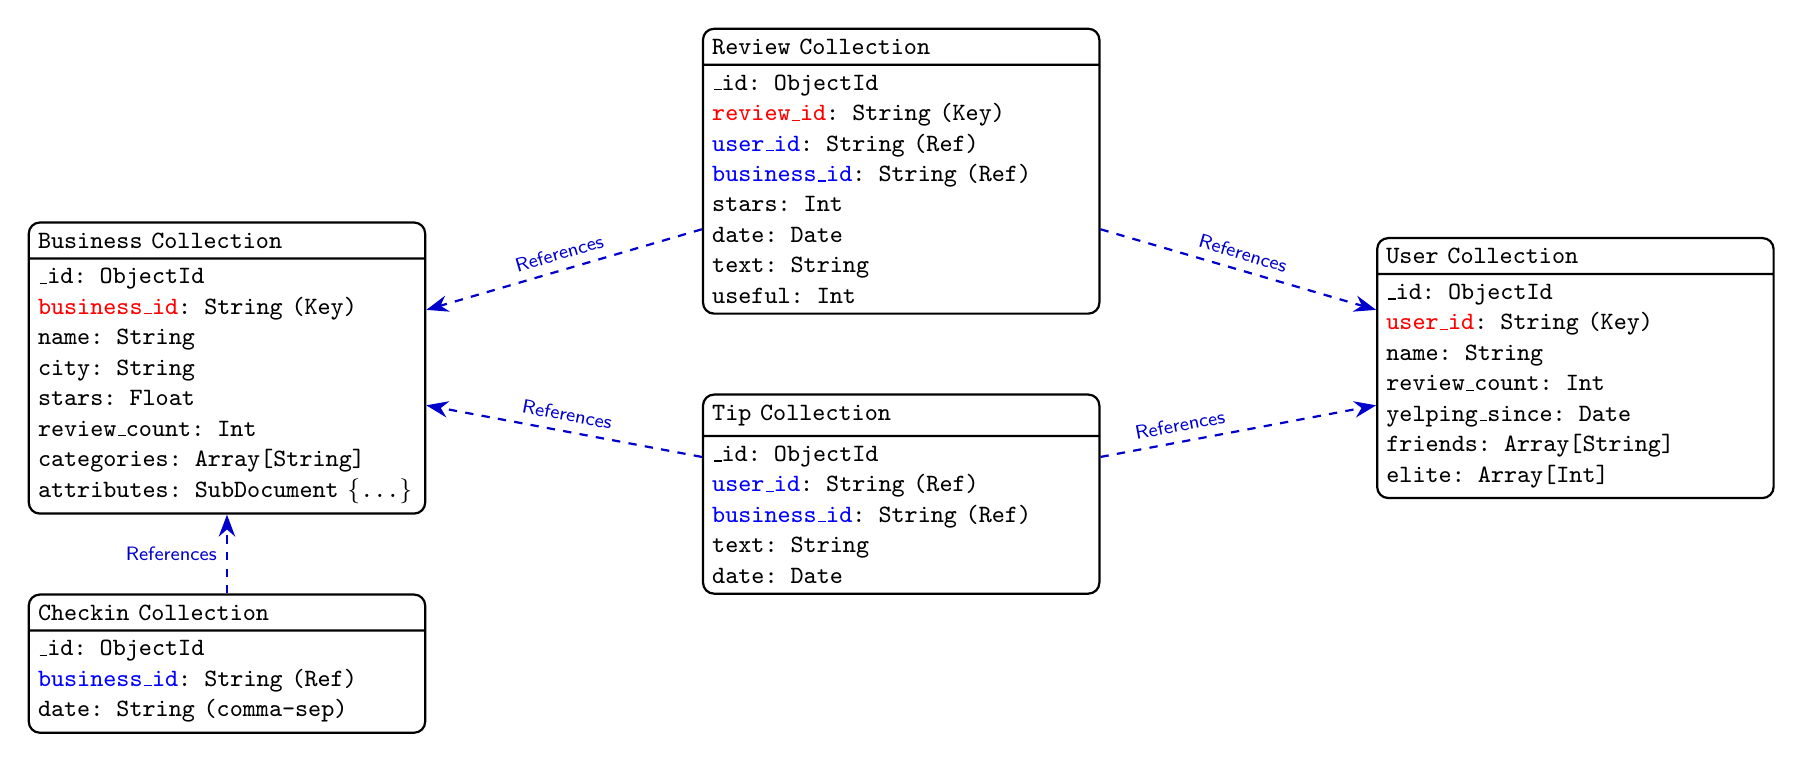
\begin{tikzpicture}[
    font=\ttfamily\small,
    doc/.style={
        rectangle split,
        rectangle split parts=2,
        draw=black, thick, fill=white,
        rounded corners,
        align=left,
        text width=4.8cm
    },
    refarrow/.style={-{Stealth[scale=1.2]}, thick, dashed, blue!80!black}
]

% Business
\node[doc] (business) {
    \nodepart{one} \textbf{Business Collection}
    \nodepart{two} 
    \_id: ObjectId\\
    \textcolor{red}{business\_id}: String (Key)\\
    name: String\\
    city: String\\
    stars: Float\\
    review\_count: Int\\
    categories: \textbf{Array[String]}\\
    attributes: \textbf{SubDocument \{...\}}
};

% Review
\node[doc, right=3.5cm of business, yshift=2.5cm] (review) {
    \nodepart{one} \textbf{Review Collection}
    \nodepart{two}
    \_id: ObjectId\\
    \textcolor{red}{review\_id}: String (Key)\\
    \textcolor{blue}{user\_id}: String (Ref)\\
    \textcolor{blue}{business\_id}: String (Ref)\\
    stars: Int\\
    date: Date\\
    text: String\\
    useful: Int
};

% User
\node[doc, right=3.5cm of review, yshift=-2.5cm] (user) {
    \nodepart{one} \textbf{User Collection}
    \nodepart{two}
    \_id: ObjectId\\
    \textcolor{red}{user\_id}: String (Key)\\
    name: String\\
    review\_count: Int\\
    yelping\_since: Date\\
    friends: \textbf{Array[String]}\\
    elite: \textbf{Array[Int]}
};

% Tip
\node[doc, below=1cm of review] (tip) {
    \nodepart{one} \textbf{Tip Collection}
    \nodepart{two}
    \_id: ObjectId\\
    \textcolor{blue}{user\_id}: String (Ref)\\
    \textcolor{blue}{business\_id}: String (Ref)\\
    text: String\\
    date: Date
};

% Checkin
\node[doc, below=1cm of business] (checkin) {
    \nodepart{one} \textbf{Checkin Collection}
    \nodepart{two}
    \_id: ObjectId\\
    \textcolor{blue}{business\_id}: String (Ref)\\
    date: String (comma-sep)
};

% Arrows mapping internal references
\draw[refarrow] (review) -- node[above, font=\sffamily\scriptsize, sloped] {References} (business);
\draw[refarrow] (review) -- node[above, font=\sffamily\scriptsize, sloped] {References} (user);
\draw[refarrow] (tip) -- node[above, font=\sffamily\scriptsize, sloped] {References} (business);
\draw[refarrow] (tip) -- node[above, font=\sffamily\scriptsize, sloped, pos=0.3] {References} (user);
\draw[refarrow] (checkin) -- node[left, font=\sffamily\scriptsize] {References} (business);

\end{tikzpicture}
\end{document}
